\paragraph{答:}
最初拿到这个题目的时候,我先仔细看了一遍RBAC的思路。
\begin{itemize}
	\item 总体而言,构成最基本的RBAC需要四个部分:用户、角色、权限和会话。其中用户代表着自然人,每个用户可以对应不同的角色,一个用户也可以对应多个角色(这取决于具体系统的需求),而每一种角色和某一种或多种权限关联;而用户只有通过会话才能获得相应的角色,在我理解来譬如“在注册时被分配角色”本质上就是一种会话。
	
	\item 拥有这些基本概念的RBAC是最基本的RBAC,叫做RBAC0,而在其之上还有RBAC1,RBAC2,RBAC3:RBAC1在RBAC0的基础上将角色定义为可继承的,而RBAC2则是对角色的指派增加了更多的规定譬如互斥、基数或者先决条件等,最后RBAC3其实就是把RBAC1和RBAC2进行了结合。
	
	\begin{enumerate}
		\item
		\begin{itemize}
			\item 有了这些基本概念之后,就可以开始动手了。
			
			\item 对于所做的系统,我初步的想法是做一个作文打分系统,角色有教师、学生以及管理员,学生的权限是登录和提交自己的作文,而老师的权限是查看作文并进行打分,管理员则能管理用户信息,可以查看所有的用户信息或者删除用户的信息。通过不同的权限设置前面面板控件的可用性和可见性,以达到基于角色的权限控制。
			
			\item 首先进行的是建模,首先画概念图如下:
			
			\begin{minipage}{\textwidth}
				\includepdf{ConceptualDiagram.pdf}
			\end{minipage}
			
			\newpage
			
			\item
			然后将该概念图转换为逻辑图:
			\begin{minipage}{\textwidth}
				\includepdf{LogicalDiagram.pdf}
			\end{minipage}
			
			\newpage
			
			\item
			然后将该逻辑图转换为物理图:
			\begin{minipage}{\textwidth}
				\includepdf{PhysicalDiagram.pdf}
			\end{minipage}
			
			\newpage
			
			\item 
			然后将该物理图转换为OOM:
			\begin{minipage}{\textwidth}
				\includepdf{OOM.pdf}
			\end{minipage}
			
			\newpage
			
			\item
			然后将物理图直接转换成SQL代码:
\begin{lstlisting}[language=sql]
/*===================================*/
/* DBMS name:      MySQL 5.0         */
/* Created on:     2017/5/8 22:29:36 */
/*===================================*/


drop table if exists Assignment;

drop table if exists Grade;

drop table if exists Permission;

drop table if exists Role;

drop table if exists Role_Permission;

drop table if exists User;

drop table if exists User_Role;

/*==================================*/
/* Table: Assignment                */
/*==================================*/
create table Assignment
(
assignment_id        int not null,
role_id              int not null,
content              varchar(2048),
primary key (assignment_id)
);

/*==================================*/
/* Table: Grade                     */
/*==================================*/
create table Grade
(
grade_id             int not null,
assignment_id        int not null,
primary key (grade_id)
);

/*==================================*/
/* Table: Permission                */
/*==================================*/
create table Permission
(
permission_id        int not null,
permission_name      varchar(20) not null,
primary key (permission_id)
);

/*==================================*/
/* Table: Role                      */
/*==================================*/
create table Role
(
role_id              int not null,
role_name            varchar(20) not null,
primary key (role_id)
);

/*==================================*/
/* Table: Role_Permission           */
/*==================================*/
create table Role_Permission
(
role_id              int not null,
permission_id        int not null,
primary key (role_id, permission_id)
);

/*==================================*/
/* Table: User                      */
/*==================================*/
create table User
(
userid               int not null,
username             varchar(20) not null,
password             varchar(20) not null,
primary key (userid)
);

/*==================================*/
/* Table: User_Role                 */
/*==================================*/
create table User_Role
(
userid               int not null,
role_id              int not null,
primary key (userid, role_id)
);

alter table Assignment add constraint 
FK_Role_Assignment foreign key (role_id)
references Role (role_id) on delete 
restrict on update restrict;

alter table Grade add constraint 
FK_Assignment_Grade foreign key (assignment_id)
references Assignment (assignment_id)
on delete restrict on update restrict;

alter table Role_Permission add constraint
FK_Role_Permission foreign key (role_id)
references Role (role_id) on delete 
restrict on update restrict;

alter table Role_Permission add constraint
FK_Role_Permission2 foreign key (permission_id)
references Permission (permission_id) on
delete restrict on update restrict;

alter table User_Role add constraint 
FK_User_Role foreign key (userid)
references User (userid) on delete 
restrict on update restrict;

alter table User_Role add constraint 
FK_User_Role2 foreign key (role_id)
references Role (role_id) on delete 
restrict on update restrict;
			\end{lstlisting}
			
			\newpage
			\item
			执行这一段SQL代码生成所有需要的表:
			\begin{figure}[H]
				\centering
				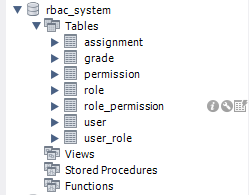
\includegraphics[width=\textwidth]{tables}
				\caption{Tables}
				\label{fig:tables}
			\end{figure}
			
			\newpage
			\item
			然后通过Hibernate的逆向工程生成相应的Entity类:
			\begin{figure}[H]
				\centering
				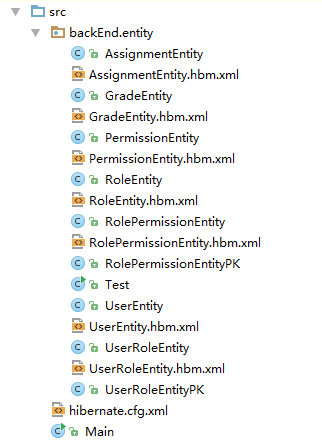
\includegraphics[width=\textwidth]{packages}
				\caption{Entities}
				\label{fig:packages}
			\end{figure}
			\item
			可是当我准备进行存取的时候,Hibernate报错了:
			\begin{figure}[H]
				\centering
				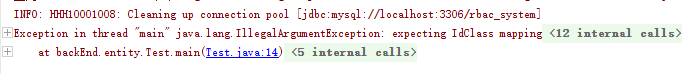
\includegraphics[width=\textwidth]{error}
				\caption{Error}
				\label{fig:error}
			\end{figure}
			
			\item
			到了最后也没有排查出来出错的原因,sign...
		\end{itemize}
	
		\item
		由于时间宝贵,我只能暂时放下这个已经快完成了后端的项目,而重新开始一个RBAC Demo。
		
		\item
		现在的想法是一个比上一个例子简单许多的Demo,想法如下:\\ 这个系统中包含了三种角色:管理员,教师和学生。管理员能查看所有的教师账户和学生账户,而教师只能查看所有的学生账户,学生不能查看别人的账户,此外,每种角色都有自己独有的按钮。系统在初始化的时候创建了一个管理员账户hello@hello.com并且系统以后也有且只有这一个管理员(因为注册选项没有注册为管理员的选项而只有教师和学生)。这次的技术选用在Android平台上。
		\begin{itemize}
			\item 
		\end{itemize}
	\end{enumerate}
	
	
\end{itemize}
